\documentclass[12 pt]{article}
\usepackage{hyperref, fancyhdr, setspace, enumerate, amsmath,
  lastpage, amssymb, algpseudocode, bussproofs, tikz, listings,
  marvosym, stmaryrd, collectbox}
\usetikzlibrary{shapes.geometric}
\usetikzlibrary{positioning}
\EnableBpAbbreviations
\usepackage[margin=1 in]{geometry}
\allowdisplaybreaks
% \usepackage[dvipsnames]{xcolor}   %May be necessary if you want to color links
\hypersetup{
  % colorlinks=true, %set true if you want colored links
  linktoc=all,     %set to all if you want both sections and subsections linked
  linkcolor=black,  %choose some color if you want links to stand out
}
% New environment to scale prooftrees, from https://tex.stackexchange.com/questions/104554/how-to-scale-prooftree-environment-bussproofs-package
\newenvironment{scprooftree}[1]%
  {\gdef\scalefactor{#1}\begin{center}\proofSkipAmount \leavevmode}%
  {\scalebox{\scalefactor}{\DisplayProof}\proofSkipAmount \end{center}
}
%New command \mybox to box something
\newcommand{\mybox}{%
\collectbox{%
	\setlength{\fboxsep}{3pt}%
	\fbox{\BOXCONTENT}%
	}%
}

\DeclareMathOperator*{\argmax}{arg\!\max}
\DeclareMathOperator*{\argmin}{arg\!\min}

\usepackage{graphicx}
\graphicspath{{Images/}}
\author{Julian Lore}
\date{Last updated: \today}
\title{MATH 423: Regression and Analysis of Variance}
\pagestyle{fancy}
\lhead{MATH 423}
\chead{\leftmark}
\rhead{Julian Lore}
\cfoot{Page \thepage \ of \pageref{LastPage}}
\newcommand{\tab}[1]{\hspace{.2\textwidth}\rlap{#1}}
\newenvironment{rcases}
  {\left.\begin{aligned}}
  {\end{aligned}\right\rbrace}
\begin{document}
\onehalfspacing
\maketitle
\tableofcontents
\section{Introduction}
\begin{itemize}
\item
\textbf{Regression analysis} is about investigating quantitative predictive
relationships variables. Several examples include: getting a car insurance quote. You
provide the company/website a lot of personal information about
yourself and your car and then they'll tell you an estimated price of
your car insurance. How do they get this estimated price? Linear
regression. Another application is estimating your time of arrival
when taking a taxi or some other ride. Credit card applications also
use some form of linear regression to assess the risk of you not
paying your debt, etc. Many asset management pricing models use linear
regression too.
\item
  \textbf{Prediction} is important, which consists of studying the
  relation between two or more variables
\item This class is about:
  \begin{itemize}
  \item Crafting predictive mathematical models
  \item Seeing whether such models really have any predictive power
  \item Comparing their predictions
  \end{itemize}
\end{itemize}
A more concrete example is Sales vs TV, Radio and Newspaper
advertising, with a linear-regression line fit for each. Now we want
to predict sales using all three variables, i.e.\ $Sales \approx
f(TV,Radio,Newspaper)$. Eventually we will study how to estimate this
function $f$ given the data.

Let's go back to a simpler example. Say we only have one variable,
with no other variables, e.g.\ temperature, we want to estimate the
temperature but only have historical data of previous
temperatures. How do we predict tomorrow's temperature? Here we
\textcolor{red}{cannot} use regression, we don't have two
variables. The simplest answer is to use an average. Get the average
of the previous temperatures of the same date of previous years. How
do we generalize this? Given multiple variables but only wanting to
predict one, how do we do so? It will still be some sort of average,
but not simply an average of the output.
\section{Statistical Prediction and\\ Optimal Linear Regression}
\subsection{Predicting a Random Variable from its Distribution}
Let's first think about what the optimal prediction would look like,
if we somehow knew all the probability distribution of our
variable. Suppose we want to predict the value of a random variable
$Y$. What's the best prediction we can make? The best one-number guess
we could make for $Y$ is just its expected value $E(Y)$. Why is this
the case? We want to mathematically show this.

We need some way to measure how good a prediction $m$ is.
\begin{itemize}
\item The difference $Y-m$ should be small
\item Since we don't care about positive more than negative errors, we
  can use $(Y-m)^2$. Since $Y$ is random, this will fluctuate (it is a
  function of a random variable and is thus also a random variable). So we
  use its expected value.
\end{itemize}
  $$MSE(m) = E[(Y-m)^2]$$
  where MSE stands for mean square error. However, sometimes the
  positive and negative error don't have the same importance, like
  predicting bank expenses, you don't want to predict negative
  expenses as you may go bankrupt. In this case the median may be
  better. We will see this case later. Also note that $(Y-m)^2$ is
  called the loss function.

  From the definition of variance:
  \begin{align*}
    MSE(m) & = E[(Y-m)^2] = (E[(Y-m)])^2 + Var[Y-m] = (E[Y]-m)^2 + Var[Y]
  \end{align*}
  We cannot control the variance of $Y$, as it is given to us. We can
  however, do something about $(E[Y] - m)^2$, thus seeing that the
  optimal solution would be $m = E[Y]$.

  But if we don't have all the data on $Y$, then we can estimate
  $E[Y]$ using the sample mean.

Say you have an infinite amount of data, but it is always fluctuating
and you cannot get a hold of a value. How should we estimate it? The
theory tells us to use the expected value. This does not rely on the
actual distribution. However, in reality, we often don't have the full
knowledge of the distribution, we often have discrete measurements,
i.e.\ a histogram. In this case we use the sample mean.

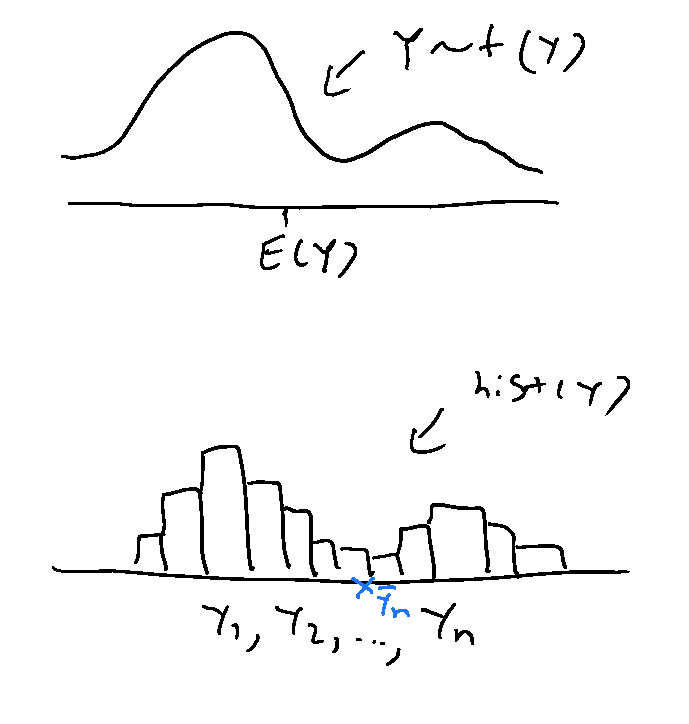
\includegraphics[width=.7\textwidth]{1.pdf}

Looking back at $(E[Y]-m)^2 + Var[Y]$, the first term is the squared
bias of estimating $Y$ with $m$. So we want to choose an $m$ such that
this bias is minimized (should be $0$, as we can set $m=Y$).

The second term is the variance of $Y-m$ (or variance of $Y$, since
$m$ is not random).

This form is called the Bias-Variance decomposition which plays a
central role in machine learning. This isn't only true for just linear
model, it's true for any random variable $Y$.

We would like to pick $m$ to make $MSE(m)$ small. Denote $m^*$ as the
value of $m$ that minimizes $MSE(m)$.
$$m^* = \argmin_m E[(Y-m)^2]$$
$Var(Y)$ is irrelevant to making this small, since it's the same no
matter what $m$ is.

To find the minimum of $MSE(m)$, we denote $\mu = E(Y)$.
\begin{align*}
  \frac{dMSE(m)}{dm} & = \frac{d}{dm} \left[Var[Y] + (\mu - m)^2\right] = \frac{dVar(Y)}{dm} + 2(\mu-m) \left(\frac{d\mu}{dm} - \frac{dm}{dm}\right)
  \\ & = 0 + 2(\mu - m) \left(0 - \frac{dm}{dm}\right) = - 2(\mu - m) = 0
\end{align*}
Therefore
$$m^* = \mu = E(Y)$$
In other words, the best one number guess for $Y$ is just $E(Y)$.

\subsection{Two Variables/Predicting one random variable from another}
Now what about the case in which we have $X$ and $Y$, two random
variables that we can collect data from. Just using the expected value
of $Y$ (say insurance claim) is not fair for the different $x$ (say
age), as everyone will pay the same rate even though different age
groups have different average insurance claims. So we look around a
certain age group using conditional probability, i.e.\ $E[Y|X =
40]$. So we can do this for every value of $X$ and then we get a
\textbf{regression line}.

More formally: we have two random variables, $X$ and $Y$ and their
joint distribution.
\\ We use $X$ to predict $Y$. Our prediction is therefore a function
of $X$, which we'll denote as $m(x)$. What's the best prediction we
can get?
$$m^*(x) = E[Y | X = x]$$
Using the same criterion as the single variable case, we want to
minimize:
$$m^*(\cdot) = \argmin_{m(\cdot)} E_{X,Y}[(Y-m(x))^2]$$
If we denote $\mu(x) = E_{Y|X}[Y|X = x]$ to represent the conditional
expectation of $Y$ given $X = x$. We will prove that
$$m^*(x) = \mu(x)$$
\paragraph{Proof:}
\begin{align*}
  E_{X,Y}[(Y-m(x))^2] & = E_{X}[E_{Y|X}[(Y-m(x))^2 | X]]
\end{align*}

We can call the left hand side the loss function, or the
generalization error.

For the inner expectation, for each possible value of $X = x$, the
optimal value $m^*(x)$ is just the conditional mean (since $x$ is a
constant when conditioned on):
$$m^*(x) = \mu(x) = \underbrace{E_{Y|X}[Y|X = x]}_{\text{regression function}}$$

In terms of estimation, if you want to get the optimal value at $X=4$,
you need lots of observations at $X=4$ to approximate the expected
value of $Y$ given $X = 4$. If we don't have lots of observations, we
use the point's $k$-nearest neighborhood, include extra points around $X =
4$ to estimate the expectation. This performs pretty well in
general. However in the higher dimension cases, a small neighborhood
will include less points, so you have less points to average and might
not be able to use this method.
\paragraph{$k$-nearest neighborhood (KNN)} (side topic, not directly related
to linear regression, but very important, linear regression is the
strictest model, whereas the nearest neighborhood model is the least
strict, you don't rely on a distribution or anything, whereas the
linear regression model relies heavily on a distribution)

Goal: to estimate the conditional distribution of $Y$ given $X$. $X
\in \mathbb{R}^p$, $p \geq 1$ (i.e.\ $X$ can be higher dimensional, a
vector). Specifically, $E[Y | X = x]$. Given a positive integer $K$
and a test observation $x_0$, the procedure is as follows.
\\ Procedure: KNN
\begin{itemize}
\item First identify $K$ points in the training data that are closest
  to $x_0$, represented by $N_0$.
\item Then estimate $$\hat{E}[Y | X = x_0] = \frac{1}{k} \sum_{i \in N_0}y_i$$
  (the hat signifies an estimation)
\end{itemize}
\paragraph{Example}
\begin{tabular}{l l l l l}
  \hline Observation& $X_1$& $X_2$&$X_3$&$Y$
  \\ \hline $x_1$ & $0$ & $3$ & $0$ & $1$
  \\ $x_2$ & $2$ & $0$ & $0$ & $2$
  \\ $x_3$ & $0$ & $1$ & $3$ & $3$
  \\ $x_4$ & $0$ & $1$ & $2$ & $4$
  \\ $x_5$ & $-1$ & $0$ & $1$ & $5$
  \\ $x_6$ & $1$ & $1$ & $1$ & $6$
\end{tabular} This is our \textbf{training data}.
\\ Suppose we want to use this data set to make a prediction for $Y$
when $x = (x_{01}, x_{02}, x_{03}) = (0, 0,0)$ using $K$-NN.\
\begin{enumerate}[(a)]
\item Compute the Euclidean distance between each observation and the
  test point, $x_0$.
  \begin{itemize}
  \item $\left\lVert x_1 - x_0 \right\rVert_2 = \sqrt{(0-0)^2 +
      (3-0)^2 + (0-0)^2} = 3$
  \item $\left\lVert x_2 - x_0 \right\rVert_2 = 2$
  \item $\left\lVert x_3 - x_0 \right\rVert_2 = \sqrt{10}$
  \item $\left\lVert x_4 - x_0 \right\rVert_2 = \sqrt{5}$
  \item $\left\lVert x_5 - x_0 \right\rVert_2 = \sqrt{2}$
  \item $\left\lVert x_6 - x_0 \right\rVert_2 = \sqrt{3}$
  \end{itemize}
\item Now we can get a prediction for any hyper parameter $k$. What is
  the prediction with $k = 1$? $x_5$ is closest to $x_0$ so our
  prediction is $Y = 5$.
\item $k = 3$, $\frac{1}{3} (2 + 5 + 6) = \frac{13}{3}= 4 \frac{1}{3}$
\end{enumerate}
So this method is very flexible as it does not rely on any
distribution. However, it becomes very difficult to find the optimal
$k$ and the performance of the algorithm gets worse as we increase the
dimension. Though in many cases, this is still the best method to
use. Often people use a combination of this method and linear models.

\subsection{The Optimal Linear Predictor}
Unfortunately, in general $m(x)$ is a really complicated function for
which there exists no nice mathematical expression. We could
substitute a simplified model for the relationship for
the actual relation.

We restrict the prediction function $m(x)$ to have the linear form,
i.e.\ $$m(x) = \beta_0 + \beta_1 x$$
Now we want to know what the optimal prediction we can make which is
linear in $X$?

To minimize the mean squared error of $m(x) = \beta_0 + \beta_1 x$
\begin{align*}
  (\beta_0^*, \beta_1^*) & = \argmin_{(\beta_0,, \beta_1)} E_{X, Y}[(Y - \underbrace{(\beta_0 + \beta_1 x)}_{m(x)})^2]
  \\ E[(Y - (\beta_0 + \beta_1 x))^2] & = E[Y^2] - 2 \beta_0 E[Y] - 2 \beta_1 E[XY] + E [ (\beta_0 + \beta_x)]
  \\ & = E [Y^2] - \beta_0 E[Y] -  \beta_1 (Cov (X,Y)) + E[X]E[Y] + \beta_0^2 + 2\beta_0\beta_1 E[X] + \beta_1^2 E[X]
  \\ & = E[Y^2] - 2 \beta_0 E[Y] - 2 \beta_1 (Cov(X,Y)) + E[X]E[Y] + \beta_0^2 + 2 \beta_0 \beta_1 E[X]
  \\ & + \beta_1^2 (Var(X) + E[X]^2)
\end{align*}
Now to get the optimal values, we take the derivative:
\begin{align*}
  \frac{\partial{E[Y - (\beta_0+\beta_1X)^2]}}{\partial{\beta_0}} & = -2E[Y] + 2 \beta_0 + 2\beta_1 E[X] = 0
\end{align*}
This gives us:
$$\beta_0^* = E[Y] - \beta_1^* E[X] \iff E[Y] = \beta_0^* + \beta_1^*
E[X]$$
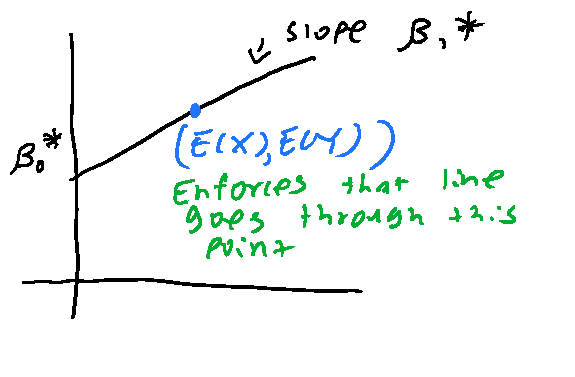
\includegraphics[width=.9\textwidth]{2.pdf}
\begin{itemize}
\item The optimal intercept $\beta_0^*$ ensures that the line goes
  through $E[Y]$ at the $E[X]$ value.
\item If the variables were centered with $E[Y] = E[X] = 0$ then
  $\beta_0^* = 0$.
\end{itemize}
\begin{align*}
  \frac{\partial{E[Y]-(\beta_0+\beta_1X)^2}}{\partial{\beta_1}} & = -2Cov(X,Y) - 2E[X]E[Y] + 2\beta_0E[X] + 2\beta_1 Var(X) + 2\beta_1 (E[X])^2
                                                                  \intertext{Plug
                                                                  in
                                                                  $\beta_0^*
                                                                  =
                                                                  E[Y]
                                                                  -
                                                                  \beta_1^*
                                                                  E[X]$}
  & = -Cov(X,Y) + \beta_1 Var(X) = 0
  \\ \beta_1^* & = \dfrac{Cov(X,Y)}{Var(X)}
\end{align*}
\begin{itemize}
\item Since the optimal slope $\beta_1^*$ is $\frac{Cov(X,Y)}{Var(X)}$
  (ratio), the slope increases the more $X$ and $Y$ tend to fluctuate
  together, and gets smaller/closer to zero the more $X$ fluctuates.
  \\ 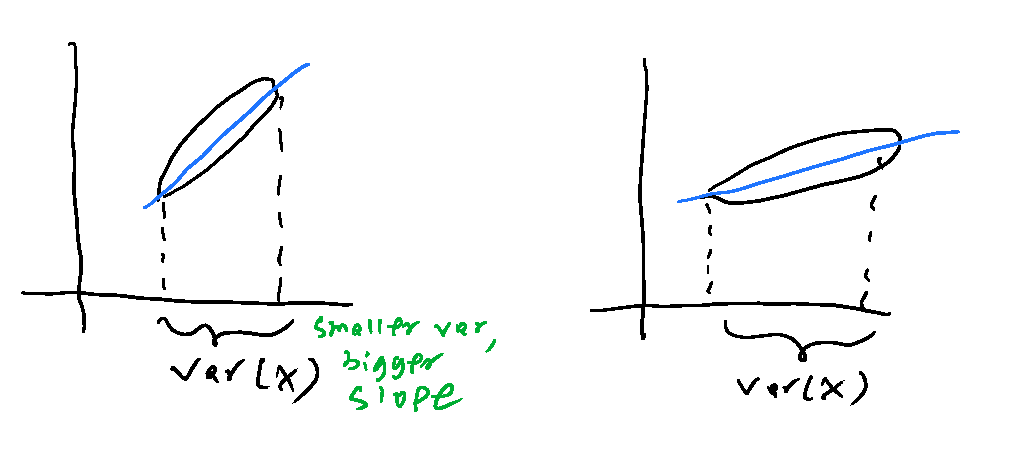
\includegraphics[width=.9\textwidth]{3.pdf}
\item $\beta_1^*$ doesn't change if we use $X' = X-a, Y' = Y - b$
  instead. Note that $a$ and $b$ must be deterministic/non-random.
\end{itemize}
Eventually you will get the \textbf{optimal regression line} (of $Y$
on $X$):
$$m^*(X) = \beta_0^* + \beta_1^* X$$
\begin{itemize}
\item At no time did we have to assume that the actual relationship
  between $X$ and $Y$ is linear (that's just our belief, it may not
  actually be linear). We only have an optimal linear approximation to
  the \textbf{true relationship}, whatever it might be. Your data
  might even look like:
  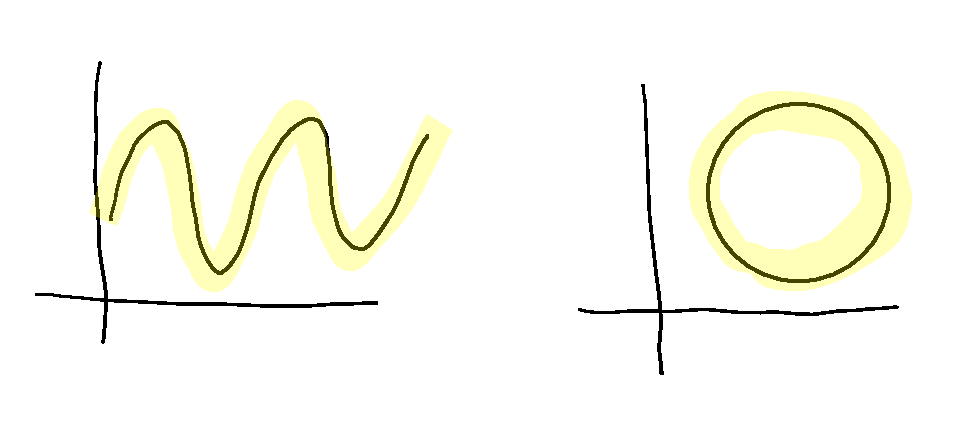
\includegraphics[width=.9\textwidth]{4.pdf}
  % \\ However, in this case linear regression will fail and a more
  % general method is required.
\item The best linear approximation to the truth can be awful. Imagine
  $$E[Y | X = x] = e^x \text{ or } \sin(X)$$
  There is no general reason to think linear approximation ought to be
  good. But \underline{sometimes} it works. For example, the true
  regression function of the above would be $E[Y | X = x] = e^x$,
  which is differentiable and can be approximated using a polynomial
  of $X$ (Taylor expansion).
  \begin{align*}
    e^x & = e^{x_0}+ \frac{de^X}{dx} \vline_{x = x_0}(x - x_0) + \frac{1}{2} \frac{d^2e^x}{dx^2}\vline_{x = x_0} (x-x_0)^2 + \ldots
    \\ & = e^{x_0} + e^{x_0}(x-x_0) + \frac{1}{2}e^{x_0}(x-x_0)^2 + \ldots
  \end{align*}
\item If $x$ is close enough to $x_0$ then $$e^x \approx e^{x_0} +
  e^{x_0}(x-x_0) = e^{x_0} (1- x_0) + e^{x_0}x$$
  In this case our linear approximation would just be the first two
  terms.

  How close is close enough? The first two terms should dominate the
  remaining terms (quadratic cubic), i.e.
  $$e^{x_0} |x - x_0| >> \frac{1}{2} e^{x_0} |x - x_0|^2 \iff 2
  \frac{e^{x_0}}{e^{x_0}} >> \frac{|x-x_0|^2}{|x-x_0|} \iff 2 >> |x -
  x_0|$$
  So $x \in (x_0 - 2, x_0 + 2)$ at least.
\end{itemize}
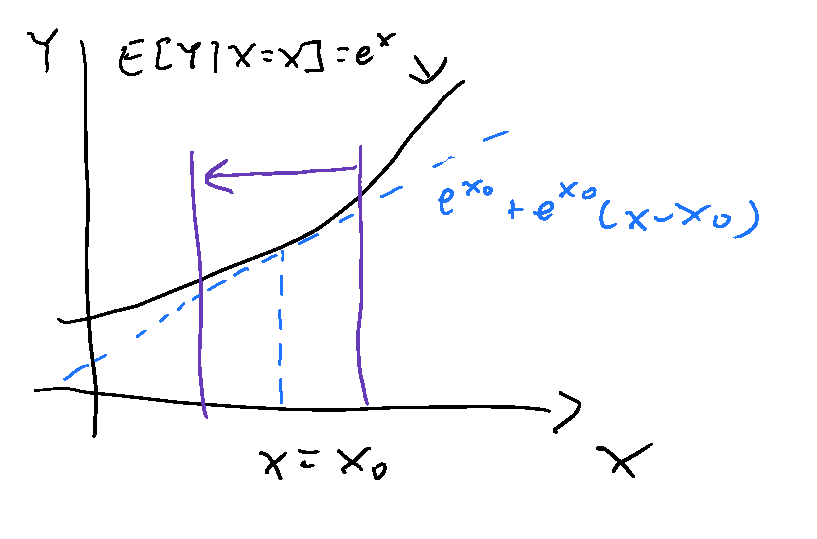
\includegraphics[width=.9\textwidth]{5.pdf}
\begin{itemize}
\item
Linear regression isn't always the best method of approximation,
however it is easy to do and is one of the main methods that is
computationally efficient for high dimension problems or if you want
to approximate many points, sometimes more than the number of
observations you have.
\item We don't assume that $X$ came before $Y$ in time, that $X$
  causes $Y$ or that $X$ is known precisely but $Y$ only noisily to
  get the optimal linear prediction.
\item At no time did we have to specify the marginal distribution of
  $X$ and $Y$, or about the joint distribution of $X$ and $Y$.
\item At no time did we have to assume anything about the fluctuation
  of $Y$ being Gaussian or symmetric.
\end{itemize}
\section{Simple Linear Regression Model}
\subsection{Notation}
We consider two types of variables.
\begin{itemize}
\item ``Output'': $Y$ \hbox{--} measured outcome of interest. Can also be
  called outcome or response variable.
\item ``Input'': $X$ \hbox{--} variable(s) that correlated to the variation in
  the ``Output''. Can also be called features, covariates/factors or
  predictors.
\end{itemize}
Both variables will be measured during the study.
\subsection{Model Setup}
The simple linear regression has two variables $X$ and $Y$ where we
try to predict $Y$ from $X$. The assumptions of the model are as
follows (this definition is more general than the one in the textbook,
however we will see a more developed one more comparable to the
textbook later):
\begin{enumerate}
\item The distribution of $Y$ is arbitrary (and perhaps $X$ is
  non-random)
\item If $X = x$ (it is given/we observe a value of $x$), then $Y =
  \beta_0 + \beta_1 x + \varepsilon$ for some constants $\beta_0$ and
  $\beta_1$ and some random noise.
  \\ Why not just use $Y = \beta_0 + \beta_1 x$? Often the
  relationship between two variables is not deterministic, for
  example, the effects of smoking can vary from person to person,
  although they may have the same value for $x$ (like age).
\item $E[\varepsilon \mid X = x] = 0$ and $Var(\varepsilon \mid X = x) =
  \sigma^2 > 0$ (constant).
\item $\varepsilon$ is uncorrelated with $X$ (i.e.\ $Cov(\varepsilon,
  X) = 0$) and is \textbf{uncorrelated across observations}.
\end{enumerate}
Note that:
\begin{enumerate}
\item The assumption is equivalent to assuming that the
  \textbf{regression function is linear}.
  \begin{align*}
  E[Y \mid X = x] & = E [\beta_0 + \beta_1 X + \varepsilon | X = x] =
                    \beta_0 + \beta_1x
    \\ Var[Y \mid X = x] & = Var[\underbrace{\beta_0+\beta_1X}_{\text{constant} \implies Var = 0} + \varepsilon \mid X = x ] = Var[\varepsilon \mid X = x] = \sigma^2
  \end{align*}
\item The noise variable $\varepsilon$ may represent
  \textbf{measurement error or fluctuation} in $Y$ or some combination
  of both.
\item The assumption of additive noise ($\varepsilon$ is just added to
  the function) is non-trivial \hbox{--} it's
  not absurd to imagine that it could be multiplicative.
\item \textbf{Linear functional form}, constant variance is not
  trivial.
\item But the assumption that noise has mean $0$ is trivial.
  \begin{align*}
    E [\varepsilon \mid X = x] & = c,\ \varepsilon' = \varepsilon - c,\ E[\varepsilon' \mid X = x] = 0
    \\ \implies Y & = (\beta_0 + c) + \beta_1 x + \varepsilon'
  \end{align*}
\end{enumerate}
With multiple data points $(X_1, Y_1), (X_2,Y_2), \ldots, (X_n,Y_n)$
(capitalized, these could be different random variables/different distributions)
then the model says that for each $i = 1, \ldots, n$
$$Y_i = \beta_0 +\beta_1 X_i + \varepsilon_i$$
where the noise variable $\varepsilon_i$ all have the same expectation
($0$) and same variance ($\sigma^2$) and $Cov(\varepsilon_i,
\varepsilon_j) = 0$ for $i \neq j$ (uncorrelated across observations
as mentioned earlier). $Cov(\varepsilon_i, \varepsilon_i) =
Var(\varepsilon_i) = \sigma^2$
\\ Equivalently, the assumption says that $E[Y_i \mid X_i = x_i] =
\beta_0 +\beta_1 x_i$ for $i = 1, \ldots, n$ and constant variance
across $i$ $$Var(Y_i \mid X_i = x_i) = \sigma^2$$ for $i = 1, \ldots, n$
\end{document}